\PassOptionsToPackage{unicode=true}{hyperref} % options for packages loaded elsewhere
\PassOptionsToPackage{hyphens}{url}
%
\documentclass[12pt,brazil,]{article}
\usepackage{lmodern}
\usepackage{setspace}
\setstretch{1.0}
\usepackage{amssymb,amsmath}
\usepackage{ifxetex,ifluatex}
\usepackage{fixltx2e} % provides \textsubscript
\ifnum 0\ifxetex 1\fi\ifluatex 1\fi=0 % if pdftex
  \usepackage[T1]{fontenc}
  \usepackage[utf8]{inputenc}
  \usepackage{textcomp} % provides euro and other symbols
\else % if luatex or xelatex
  \usepackage{unicode-math}
  \defaultfontfeatures{Ligatures=TeX,Scale=MatchLowercase}
\fi
% use upquote if available, for straight quotes in verbatim environments
\IfFileExists{upquote.sty}{\usepackage{upquote}}{}
% use microtype if available
\IfFileExists{microtype.sty}{%
\usepackage[]{microtype}
\UseMicrotypeSet[protrusion]{basicmath} % disable protrusion for tt fonts
}{}
\IfFileExists{parskip.sty}{%
\usepackage{parskip}
}{% else
\setlength{\parindent}{0pt}
\setlength{\parskip}{6pt plus 2pt minus 1pt}
}
\usepackage{hyperref}
\hypersetup{
            pdftitle={Título do meu relatório (html\_pdf\_document)},
            pdfauthor={Cristian Villegas (clobos@usp.br)},
            pdfborder={0 0 0},
            breaklinks=true}
\urlstyle{same}  % don't use monospace font for urls
\usepackage[left=3cm, right=3cm, top=2.5cm, bottom=2.5cm]{geometry}
\usepackage{color}
\usepackage{fancyvrb}
\newcommand{\VerbBar}{|}
\newcommand{\VERB}{\Verb[commandchars=\\\{\}]}
\DefineVerbatimEnvironment{Highlighting}{Verbatim}{commandchars=\\\{\}}
% Add ',fontsize=\small' for more characters per line
\usepackage{framed}
\definecolor{shadecolor}{RGB}{42,33,28}
\newenvironment{Shaded}{\begin{snugshade}}{\end{snugshade}}
\newcommand{\AlertTok}[1]{\textcolor[rgb]{1.00,1.00,0.00}{#1}}
\newcommand{\AnnotationTok}[1]{\textcolor[rgb]{0.00,0.40,1.00}{\textbf{\textit{#1}}}}
\newcommand{\AttributeTok}[1]{\textcolor[rgb]{0.74,0.68,0.62}{#1}}
\newcommand{\BaseNTok}[1]{\textcolor[rgb]{0.27,0.67,0.26}{#1}}
\newcommand{\BuiltInTok}[1]{\textcolor[rgb]{0.74,0.68,0.62}{#1}}
\newcommand{\CharTok}[1]{\textcolor[rgb]{0.02,0.61,0.04}{#1}}
\newcommand{\CommentTok}[1]{\textcolor[rgb]{0.00,0.40,1.00}{\textbf{\textit{#1}}}}
\newcommand{\CommentVarTok}[1]{\textcolor[rgb]{0.74,0.68,0.62}{#1}}
\newcommand{\ConstantTok}[1]{\textcolor[rgb]{0.74,0.68,0.62}{#1}}
\newcommand{\ControlFlowTok}[1]{\textcolor[rgb]{0.26,0.66,0.93}{\textbf{#1}}}
\newcommand{\DataTypeTok}[1]{\textcolor[rgb]{0.74,0.68,0.62}{\underline{#1}}}
\newcommand{\DecValTok}[1]{\textcolor[rgb]{0.27,0.67,0.26}{#1}}
\newcommand{\DocumentationTok}[1]{\textcolor[rgb]{0.00,0.40,1.00}{\textit{#1}}}
\newcommand{\ErrorTok}[1]{\textcolor[rgb]{1.00,1.00,0.00}{\textbf{#1}}}
\newcommand{\ExtensionTok}[1]{\textcolor[rgb]{0.74,0.68,0.62}{#1}}
\newcommand{\FloatTok}[1]{\textcolor[rgb]{0.27,0.67,0.26}{#1}}
\newcommand{\FunctionTok}[1]{\textcolor[rgb]{1.00,0.58,0.35}{\textbf{#1}}}
\newcommand{\ImportTok}[1]{\textcolor[rgb]{0.74,0.68,0.62}{#1}}
\newcommand{\InformationTok}[1]{\textcolor[rgb]{0.00,0.40,1.00}{\textbf{\textit{#1}}}}
\newcommand{\KeywordTok}[1]{\textcolor[rgb]{0.26,0.66,0.93}{\textbf{#1}}}
\newcommand{\NormalTok}[1]{\textcolor[rgb]{0.74,0.68,0.62}{#1}}
\newcommand{\OperatorTok}[1]{\textcolor[rgb]{0.74,0.68,0.62}{#1}}
\newcommand{\OtherTok}[1]{\textcolor[rgb]{0.74,0.68,0.62}{#1}}
\newcommand{\PreprocessorTok}[1]{\textcolor[rgb]{0.74,0.68,0.62}{\textbf{#1}}}
\newcommand{\RegionMarkerTok}[1]{\textcolor[rgb]{0.74,0.68,0.62}{#1}}
\newcommand{\SpecialCharTok}[1]{\textcolor[rgb]{0.02,0.61,0.04}{#1}}
\newcommand{\SpecialStringTok}[1]{\textcolor[rgb]{0.02,0.61,0.04}{#1}}
\newcommand{\StringTok}[1]{\textcolor[rgb]{0.02,0.61,0.04}{#1}}
\newcommand{\VariableTok}[1]{\textcolor[rgb]{0.74,0.68,0.62}{#1}}
\newcommand{\VerbatimStringTok}[1]{\textcolor[rgb]{0.02,0.61,0.04}{#1}}
\newcommand{\WarningTok}[1]{\textcolor[rgb]{1.00,1.00,0.00}{\textbf{#1}}}
\usepackage{longtable,booktabs}
% Fix footnotes in tables (requires footnote package)
\IfFileExists{footnote.sty}{\usepackage{footnote}\makesavenoteenv{longtable}}{}
\usepackage{graphicx,grffile}
\makeatletter
\def\maxwidth{\ifdim\Gin@nat@width>\linewidth\linewidth\else\Gin@nat@width\fi}
\def\maxheight{\ifdim\Gin@nat@height>\textheight\textheight\else\Gin@nat@height\fi}
\makeatother
% Scale images if necessary, so that they will not overflow the page
% margins by default, and it is still possible to overwrite the defaults
% using explicit options in \includegraphics[width, height, ...]{}
\setkeys{Gin}{width=\maxwidth,height=\maxheight,keepaspectratio}
\setlength{\emergencystretch}{3em}  % prevent overfull lines
\providecommand{\tightlist}{%
  \setlength{\itemsep}{0pt}\setlength{\parskip}{0pt}}
\setcounter{secnumdepth}{5}
% Redefines (sub)paragraphs to behave more like sections
\ifx\paragraph\undefined\else
\let\oldparagraph\paragraph
\renewcommand{\paragraph}[1]{\oldparagraph{#1}\mbox{}}
\fi
\ifx\subparagraph\undefined\else
\let\oldsubparagraph\subparagraph
\renewcommand{\subparagraph}[1]{\oldsubparagraph{#1}\mbox{}}
\fi

% set default figure placement to htbp
\makeatletter
\def\fps@figure{htbp}
\makeatother

\ifnum 0\ifxetex 1\fi\ifluatex 1\fi=0 % if pdftex
  \usepackage[shorthands=off,main=brazil]{babel}
\else
  % load polyglossia as late as possible as it *could* call bidi if RTL lang (e.g. Hebrew or Arabic)
  \usepackage{polyglossia}
  \setmainlanguage[]{brazil}
\fi

\title{Título do meu relatório (html\_pdf\_document)}
\author{Cristian Villegas
(\href{mailto:clobos@usp.br}{\nolinkurl{clobos@usp.br}})}
\date{10/Jul/2021}

\begin{document}
\maketitle

{
\setcounter{tocdepth}{2}
\tableofcontents
}
\hypertarget{resumo}{%
\section*{Resumo}\label{resumo}}
\addcontentsline{toc}{section}{Resumo}

Os documentos R Markdown são totalmente reproduzíveis e usa várias
linguagens, incluindo R, Python e SQL. R Markdown oferece suporte a
dezenas de formatos de saída estáticos e dinâmicos, incluindo HTML, PDF,
Word, Beamer, slides HTML5, apostilas no estilo Tufte, livros, painéis,
aplicativos shiny, artigos científicos, sites e muito mais.

Neste minicurso de duas horas, apresentamos as principais ferramentas
para criar um relatório dinâmico dentro do Rstudio com exemplos na área
da estatística.

\newpage

\hypertarget{links}{%
\section{Alguns links}\label{links}}

\begin{itemize}
\item
  \url{https://www.rstudio.com/speakers/yihui-xie/}
\item
  \url{https://www.rstudio.com/resources/cheatsheets/}
\item
  \url{https://bookdown.org/}
\item
  \url{https://bookdown.org/yihui/rmarkdown-cookbook/}
\item
  \url{https://bookdown.org/yihui/bookdown/}
\item
  \url{https://yihui.org/knitr/}
\end{itemize}

\begin{figure}

{\centering 
\includegraphics[width=0.5\linewidth]{knit_logo} 

}

\caption{Knitr logo}\label{fig:unnamed-chunk-3}
\end{figure}

\hypertarget{fuxf3rmulas}{%
\subsection{Fórmulas}\label{fuxf3rmulas}}

Veja \(f(x)=x^2\)

\hypertarget{cuxf3digo-r}{%
\subsection{Código R}\label{cuxf3digo-r}}

\begin{Shaded}
\begin{Highlighting}[]
\KeywordTok{names}\NormalTok{(airquality)}
\end{Highlighting}
\end{Shaded}

\begin{verbatim}
**--** [1] "Ozone"   "Solar.R" "Wind"    "Temp"    "Month"   "Day"
\end{verbatim}

\begin{Shaded}
\begin{Highlighting}[]
\KeywordTok{summary}\NormalTok{(airquality)}
\end{Highlighting}
\end{Shaded}

\begin{verbatim}
**--**      Ozone           Solar.R           Wind             Temp      
**--**  Min.   :  1.00   Min.   :  7.0   Min.   : 1.700   Min.   :56.00  
**--**  1st Qu.: 18.00   1st Qu.:115.8   1st Qu.: 7.400   1st Qu.:72.00  
**--**  Median : 31.50   Median :205.0   Median : 9.700   Median :79.00  
**--**  Mean   : 42.13   Mean   :185.9   Mean   : 9.958   Mean   :77.88  
**--**  3rd Qu.: 63.25   3rd Qu.:258.8   3rd Qu.:11.500   3rd Qu.:85.00  
**--**  Max.   :168.00   Max.   :334.0   Max.   :20.700   Max.   :97.00  
**--**  NA's   :37       NA's   :7                                       
**--**      Month            Day      
**--**  Min.   :5.000   Min.   : 1.0  
**--**  1st Qu.:6.000   1st Qu.: 8.0  
**--**  Median :7.000   Median :16.0  
**--**  Mean   :6.993   Mean   :15.8  
**--**  3rd Qu.:8.000   3rd Qu.:23.0  
**--**  Max.   :9.000   Max.   :31.0  
**--** 
\end{verbatim}

\begin{Shaded}
\begin{Highlighting}[]
\KeywordTok{pairs}\NormalTok{(airquality,}\DataTypeTok{col=}\StringTok{"blue"}\NormalTok{, }\DataTypeTok{pch=}\DecValTok{20}\NormalTok{,}
      \DataTypeTok{panel =}\NormalTok{ panel.smooth, }\DataTypeTok{lwd=}\DecValTok{3}\NormalTok{, }\DataTypeTok{lower.panel =} \OtherTok{NULL}\NormalTok{)}
\end{Highlighting}
\end{Shaded}

\begin{figure}
\centering
\includegraphics{html_pdf_document_files/figure-latex/unnamed-chunk-4-1.pdf}
\caption{Gráfico de dispersão qualidade do ar}
\end{figure}

A seguir uma lista de opções do \texttt{chunk}

\begin{Shaded}
\begin{Highlighting}[]
\KeywordTok{names}\NormalTok{(knitr}\OperatorTok{::}\NormalTok{opts_chunk}\OperatorTok{$}\KeywordTok{get}\NormalTok{())}
\end{Highlighting}
\end{Shaded}

\begin{verbatim}
**--**  [1] "eval"          "echo"          "results"       "tidy"         
**--**  [5] "tidy.opts"     "collapse"      "prompt"        "comment"      
**--**  [9] "highlight"     "strip.white"   "size"          "background"   
**--** [13] "cache"         "cache.path"    "cache.vars"    "cache.lazy"   
**--** [17] "dependson"     "autodep"       "cache.rebuild" "fig.keep"     
**--** [21] "fig.show"      "fig.align"     "fig.path"      "dev"          
**--** [25] "dev.args"      "dpi"           "fig.ext"       "fig.width"    
**--** [29] "fig.height"    "fig.env"       "fig.cap"       "fig.scap"     
**--** [33] "fig.lp"        "fig.subcap"    "fig.pos"       "out.width"    
**--** [37] "out.height"    "out.extra"     "fig.retina"    "external"     
**--** [41] "sanitize"      "interval"      "aniopts"       "warning"      
**--** [45] "error"         "message"       "render"        "ref.label"    
**--** [49] "child"         "engine"        "split"         "include"      
**--** [53] "purl"          "crop"
\end{verbatim}

A seguir uma lista de opções do \texttt{chunk}

\begin{Shaded}
\begin{Highlighting}[]
\NormalTok{knitr}\OperatorTok{::}\NormalTok{knit_theme}\OperatorTok{$}\KeywordTok{get}\NormalTok{()}
\end{Highlighting}
\end{Shaded}

\begin{verbatim}
**--**  [1] "acid"              "aiseered"          "andes"            
**--**  [4] "anotherdark"       "autumn"            "baycomb"          
**--**  [7] "bclear"            "biogoo"            "bipolar"          
**--** [10] "blacknblue"        "bluegreen"         "breeze"           
**--** [13] "bright"            "camo"              "candy"            
**--** [16] "clarity"           "dante"             "darkblue"         
**--** [19] "darkbone"          "darkness"          "darkslategray"    
**--** [22] "darkspectrum"      "default"           "denim"            
**--** [25] "dusk"              "earendel"          "easter"           
**--** [28] "edit-anjuta"       "edit-eclipse"      "edit-emacs"       
**--** [31] "edit-flashdevelop" "edit-gedit"        "edit-jedit"       
**--** [34] "edit-kwrite"       "edit-matlab"       "edit-msvs2008"    
**--** [37] "edit-nedit"        "edit-vim-dark"     "edit-vim"         
**--** [40] "edit-xcode"        "ekvoli"            "fine_blue"        
**--** [43] "freya"             "fruit"             "golden"           
**--** [46] "greenlcd"          "greyscale0"        "greyscale1"       
**--** [49] "greyscale2"        "kellys"            "leo"              
**--** [52] "lucretia"          "manxome"           "maroloccio"       
**--** [55] "matrix"            "moe"               "molokai"          
**--** [58] "moria"             "navajo-night"      "navy"             
**--** [61] "neon"              "night"             "nightshimmer"     
**--** [64] "nuvola"            "olive"             "orion"            
**--** [67] "oxygenated"        "pablo"             "peaksea"          
**--** [70] "print"             "rand01"            "rdark"            
**--** [73] "relaxedgreen"      "rootwater"         "seashell"         
**--** [76] "solarized-dark"    "solarized-light"   "tabula"           
**--** [79] "tcsoft"            "vampire"           "whitengrey"       
**--** [82] "xoria256"          "zellner"           "zenburn"          
**--** [85] "zmrok"
\end{verbatim}

A seguir um gráfico de dispersão dos nossos dados\ldots{}(Veja Figura
\ref{scatterplot})

\begin{Shaded}
\begin{Highlighting}[]
\KeywordTok{plot}\NormalTok{(Ozone}\OperatorTok{~}\NormalTok{Wind, }\DataTypeTok{data=}\NormalTok{airquality, }\DataTypeTok{pch=}\DecValTok{20}\NormalTok{, }
     \DataTypeTok{col=}\StringTok{"darkorange"}\NormalTok{, }\DataTypeTok{lwd=}\DecValTok{3}\NormalTok{)}
\end{Highlighting}
\end{Shaded}

\begin{figure}
\centering
\includegraphics{html_pdf_document_files/figure-latex/unnamed-chunk-7-1.pdf}
\caption{\label{scatterplot}Titulo do meu gráfico}
\end{figure}

A seguir o ajuste do modelo usando o \textcolor{red}{software R}

\begin{Shaded}
\begin{Highlighting}[]
\NormalTok{ajuste<-}\StringTok{ }\KeywordTok{lm}\NormalTok{(Ozone}\OperatorTok{~}\NormalTok{Wind, }\DataTypeTok{data=}\NormalTok{airquality)}
\NormalTok{teta<-}\StringTok{ }\KeywordTok{round}\NormalTok{(}\KeywordTok{coef}\NormalTok{(ajuste),}\DecValTok{3}\NormalTok{)}
\NormalTok{betaS<-}\StringTok{ }\KeywordTok{round}\NormalTok{(}\KeywordTok{coef}\NormalTok{(}\KeywordTok{summary}\NormalTok{(ajuste)),}\DecValTok{3}\NormalTok{)}
\NormalTok{knitr}\OperatorTok{::}\KeywordTok{kable}\NormalTok{(betaS, }\DataTypeTok{caption =} \StringTok{"}\CharTok{\textbackslash{}\textbackslash{}}\StringTok{label\{tabelajuste\}}
\StringTok{             Ajuste de um ML para os dados airquality"}\NormalTok{)}
\end{Highlighting}
\end{Shaded}

\begin{longtable}[]{@{}lrrrr@{}}
\caption{\label{tabelajuste} Ajuste de um ML para os dados
airquality}\tabularnewline
\toprule
& Estimate & Std. Error & t value &
Pr(\textgreater{}\textbar{}t\textbar{})\tabularnewline
\midrule
\endfirsthead
\toprule
& Estimate & Std. Error & t value &
Pr(\textgreater{}\textbar{}t\textbar{})\tabularnewline
\midrule
\endhead
(Intercept) & 96.873 & 7.239 & 13.383 & 0\tabularnewline
Wind & -5.551 & 0.690 & -8.040 & 0\tabularnewline
\bottomrule
\end{longtable}

O modelo ajustado foi \(\widehat{\text{Ozone}}_i=\) 96.873 -5.551
\(\text{Wind}_i\) (Veja Tabela \ref{tabelajuste})

\textcolor{red}{Alternativa}

\begin{Shaded}
\begin{Highlighting}[]
\KeywordTok{cat}\NormalTok{(}\KeywordTok{sprintf}\NormalTok{(}\StringTok{"$Ozone=%.3f %.3f Wind$"}\NormalTok{,teta[}\DecValTok{1}\NormalTok{], teta[}\DecValTok{2}\NormalTok{]))}
\end{Highlighting}
\end{Shaded}

\begin{verbatim}
**--** $Ozone=96.873 -5.551 Wind$
\end{verbatim}

Veja mais detalhes na seção \ref{links}

\hypertarget{citando-livros-artigos-etc}{%
\section{Citando livros, artigos,
etc}\label{citando-livros-artigos-etc}}

\begin{Shaded}
\begin{Highlighting}[]
\KeywordTok{citation}\NormalTok{(}\StringTok{"ggplot2"}\NormalTok{)}
\end{Highlighting}
\end{Shaded}

\begin{verbatim}
**--** 
**--** To cite ggplot2 in publications, please use:
**--** 
**--**   H. Wickham. ggplot2: Elegant Graphics for Data Analysis.
**--**   Springer-Verlag New York, 2016.
**--** 
**--** A BibTeX entry for LaTeX users is
**--** 
**--**   @Book{,
**--**     author = {Hadley Wickham},
**--**     title = {ggplot2: Elegant Graphics for Data Analysis},
**--**     publisher = {Springer-Verlag New York},
**--**     year = {2016},
**--**     isbn = {978-3-319-24277-4},
**--**     url = {https://ggplot2.tidyverse.org},
**--**   }
\end{verbatim}

Equação com numero

\begin{equation}
y_i=\beta_0 + \beta_1 x_i + \epsilon_i \label{Eq0}
\end{equation}

Veja equação (\ref{Eq0}). Podemos usar Wickham (2016) ou (Wickham 2016).

\begin{figure}

{\centering 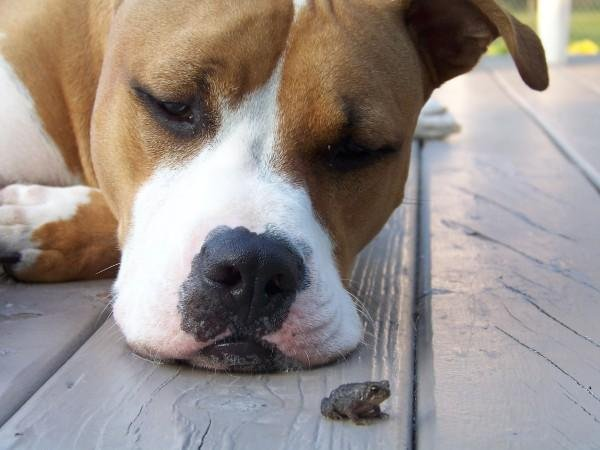
\includegraphics[width=0.5\linewidth]{cachorro} 

}

\caption{Cachorro}\label{fig:unnamed-chunk-11}
\end{figure}

\begin{equation}
y_i=\beta_0 + \beta_1 x_i + \epsilon_i,\label{Eq1}
\end{equation}

Veja equação (\ref{Eq1}).

\hypertarget{referuxeancias}{%
\section*{Referências}\label{referuxeancias}}
\addcontentsline{toc}{section}{Referências}

\hypertarget{refs}{}
\leavevmode\hypertarget{ref-ggplot2}{}%
Wickham, Hadley. 2016. \emph{ggplot2: Elegant Graphics for Data
Analysis}. Springer-Verlag New York. \url{http://ggplot2.org}.

\end{document}
